\documentclass{beamer}

\usepackage{verbatim}
\usepackage{fancyvrb}
\usepackage{amsmath}
\usepackage{mathtools}
\usepackage{booktabs}
\usepackage{amssymb}
\usepackage{graphicx}
\usepackage{calc}
\usepackage{color}
\usepackage{multicol}
\usepackage{wrapfig}
\usepackage{natbib}
\usepackage[ruled,vlined]{algorithm2e}
\usepackage{animate}
\usepackage{mathtools}
\usepackage{listings}

\usepackage{cmbright}
\fontencoding{OT1}\fontfamily{cmbr}\selectfont %to load ot1cmbr.fd
\DeclareFontShape{OT1}{cmbr}{bx}{n}{% change bx definition
<->cmbrbx10%
}{}
\normalfont % back to normalfont

% two col: two columns
\newenvironment{twocol}[4]{
\begin{columns}[c]
\column{#1\textwidth}
#3
\column{#2\textwidth}
#4
\end{columns}
}

\makeatletter
\setbeamertemplate{theorem begin}
{%
\begin{\inserttheoremblockenv}
  {}{\usebeamerfont*{block title}\usebeamercolor[fg]{block title}%
  \inserttheoremname
  %\inserttheoremnumber
  \ifx \inserttheoremaddition \empty \else\ (\inserttheoremaddition)\fi
  \inserttheorempunctuation}
  \normalfont
  }
  \setbeamertemplate{theorem end}{\end{\inserttheoremblockenv}}
\makeatother

\newcommand{\E}{\mathrm{E}}
\newcommand{\Var}{\mathrm{Var}}
\newcommand{\Cov}{\mathrm{Cov}}
\newcommand{\sd}{\mathrm{sd}}
\newcommand{\s}{\mathrm{s}}
\newcommand{\Corr}{\mathrm{Corr}}
\newcommand{\rank}{\mathrm{rank}}
\newcommand{\trace}{\mathrm{trace}}
\newcommand{\nullspace}{\mathrm{null}}
\newcommand{\myspan}{\mathrm{span}}
\DeclareMathOperator*{\argmax}{arg\,max}
\DeclareMathOperator*{\argmin}{arg\,min}
\DeclareMathOperator*{\softmax}{softmax}

\definecolor{darkgreen}{rgb}{0,0.5,0}

\newtheorem{proposition}[theorem]{Proposition}
\newtheorem{exe}{Exercise}
\newtheorem{notation}{Notation}
\newtheorem{remark}{Remark}

\definecolor{darkgreen}{rgb}{0,0.5,0}

\title{Model Selection and Validation}
\author{Zhenisbek Assylbekov}
\institute{Department of Mathematics}
\date{Regression Analysis}

\AtBeginSection[]
{
  \begin{frame}<beamer>
    \tableofcontents[currentsection]
  \end{frame}
}

\begin{document}

\begin{frame}
  \titlepage
\end{frame}

\section{Manual model selection}

\begin{frame}[fragile]{Salary example}{\url{https://github.com/zh3nis/MATH440/tree/main/chp09/salary.R}}
Model annual salary (in \$1000) as function of \begin{itemize}
    \item\pause \texttt{age} (in years),
    \item\pause \texttt{educ}ation (years of post-high-school education), and 
    \item\pause \texttt{pol}itical affiliation (\texttt{pol} = D for
Democrat, \texttt{pol} = R for Republican, and \texttt{pol} = O for other).
\end{itemize}  

\begin{footnotesize}
\pause\begin{verbatim}
> salary_data = read.table("path/to/salary.txt", header=FALSE)
> colnames(salary_data) = c('salary', 'age', 'educ', 'pol')
> head(salary_data)
  salary age educ pol
1     38  25    4   D
2     45  27    4   R
3     28  26    4   O
4     55  39    4   D
5     74  42    4   R
6     43  41    4   O
\end{verbatim}
\end{footnotesize}
\end{frame}

\begin{frame}[fragile]{Salary example}{\url{https://github.com/zh3nis/MATH440/tree/main/chp09/salary.R}}
\begin{footnotesize}
\begin{verbatim}
Coefficients:
            Estimate Std. Error t value Pr(>|t|)    
(Intercept)  17.0313     7.3459   2.318  0.03735 *  
age           0.8983     0.1968   4.565  0.00053 ***
educ          1.5039     1.1841   1.270  0.22632    
polO        -16.5404     4.8807  -3.389  0.00484 ** 
polR          9.1587     4.8482   1.889  0.08139 .  
---

Residual standard error: 8.209 on 13 degrees of freedom
Multiple R-squared:  0.8374,	Adjusted R-squared:  0.7873     
\end{verbatim}
\end{footnotesize}

\begin{itemize}
\item We can also test quadratic effects and interactions.
\item From the initial fit, \texttt{educ} is not needed with \texttt{age} and \texttt{pol} in
the model. Let's refit:
\end{itemize}

\end{frame}

\begin{frame}[fragile]
\frametitle{Droc \texttt{educ}?}
\begin{footnotesize}
\begin{verbatim}
> m2 = update(m1, . ~ . - educ)
> anova(m1, m2)
Analysis of Variance Table

Model 1: salary ~ age + educ + pol
Model 2: salary ~ age + pol
  Res.Df    RSS Df Sum of Sq      F Pr(>F)
1     13 876.03                           
2     14 984.72 -1    -108.7 1.6131 0.2263

> summary(m2)
lm(formula = salary ~ age + pol, data = salary_data)

Coefficients:
            Estimate Std. Error t value Pr(>|t|)    
(Intercept)  21.5172     6.5806   3.270  0.00559 ** 
age           1.0345     0.1686   6.136 2.58e-05 ***
polO        -16.7414     4.9838  -3.359  0.00468 ** 
polR          8.6379     4.9354   1.750  0.10196    
Residual standard error: 8.387 on 14 degrees of freedom
Multiple R-squared:  0.8172,	Adjusted R-squared:  0.778 
\end{verbatim}
\end{footnotesize}
\end{frame}

\begin{frame}[fragile]
\frametitle{Add 2nd order terms?}
\begin{footnotesize}
\begin{verbatim}
> salary_data$age2 = salary_data$age^2
> m3 = update(m2, . ~ . + age2 + age*pol)
> summary(m3)

Call:
lm(formula = salary ~ age + pol + age2 + age:pol, data = salary_data)

Coefficients:
             Estimate Std. Error t value Pr(>|t|)   
(Intercept) -20.94355   20.34047  -1.030  0.32528   
age           3.17751    0.93793   3.388  0.00606 **
polO        -16.90846   22.83050  -0.741  0.47444   
polR         -1.18699   21.44129  -0.055  0.95684   
age2         -0.02514    0.01255  -2.004  0.07037 . 
age:polO      0.05101    0.65536   0.078  0.93936   
age:polR      0.28944    0.61956   0.467  0.64950   
---
Signif. codes:  0 ‘***’ 0.001 ‘**’ 0.01 ‘*’ 0.05 ‘.’ 0.1 ‘ ’ 1

Residual standard error: 7.434 on 11 degrees of freedom
Multiple R-squared:  0.8871,	Adjusted R-squared:  0.8256 
\end{verbatim}
\end{footnotesize}
\end{frame}


\begin{frame}[fragile]{Drop 2nd order terms?}
\begin{footnotesize}
\begin{verbatim}
> anova(m3, m2)
Analysis of Variance Table

Model 1: salary ~ age + pol + age2 + age:pol
Model 2: salary ~ age + pol
  Res.Df    RSS Df Sum of Sq      F Pr(>F)
1     11 607.88                           
2     14 984.72 -3   -376.84 2.2731 0.1369    
\end{verbatim}
\end{footnotesize}
\pause We don't need \textit{all} the 2nd order terms ($p=0.137$), although there’s some indication in the table of regression effects that age$^2$ might be needed.
\pause\begin{footnotesize}
\begin{verbatim}
> anova(m4, m2)
Analysis of Variance Table

Model 1: salary ~ age + pol + age2
Model 2: salary ~ age + pol
  Res.Df    RSS Df Sum of Sq      F  Pr(>F)  
1     13 645.09                              
2     14 984.72 -1   -339.64 6.8444 0.02134 *
\end{verbatim}
\end{footnotesize}
\end{frame}

\begin{frame}[fragile]{Final model}
Our final model is 
$$
\text{salary}_i = \beta_0+\beta_1\cdot\text{age}+\beta_{2}\cdot\mathbb{I}[\text{pol}=\text{O}]+\beta_{3}\cdot\mathbb{I}[\text{pol}=\text{R}]+\beta_{4}\cdot\text{age}^2+\epsilon_i
$$
\begin{footnotesize}
\begin{verbatim}
> summary(m4)

Call:
lm(formula = salary ~ age + pol + age2, data = salary_data)

Coefficients:
              Estimate Std. Error t value Pr(>|t|)   
(Intercept) -24.751745  18.529243  -1.336  0.20452   
age           3.272388   0.867049   3.774  0.00232 **
polO        -15.891696   4.198662  -3.785  0.00227 **
polR          9.260234   4.152253   2.230  0.04399 * 
age2         -0.024576   0.009394  -2.616  0.02134 * 
---

Residual standard error: 7.044 on 13 degrees of freedom
Multiple R-squared:  0.8802,	Adjusted R-squared:  0.8434 
\end{verbatim}
\end{footnotesize}
\end{frame}

\section{Caution regarding scatterplots}

\begin{frame}{Scatterplots}
\begin{itemize}
\item Scatterplots show the \textit{marginal} relationship between $Y$ and
each of the $x_1, \ldots, x_k$. \pause They \textit{cannot} show you anything about the joint relationship among the $Y, x_1, \ldots, x_k$.
\item \pause Nonlinear relationship between $Y$ and $x_j$ ($j = 1, \ldots, k$) \textit{marginally} may or may not be present in the joint relationship.
\item \pause Actually, any strong relationship between $Y$ and $x_j$ marginally
doesn't mean that $x_j$ will be needed in the presence of other
variables.
\item \pause Seeing no marginal relationship between Y and $x_j$ does not
mean that $x_j$ is not needed in a model including other
predictors.
\end{itemize}
\end{frame}

\begin{frame}{No relationship?}
Here $Y$ vs. $x_1$ and $Y$ vs. $x_2$ shows nothing. There seems to be some multicollinearity though.
\vspace{10pt}

\centerline{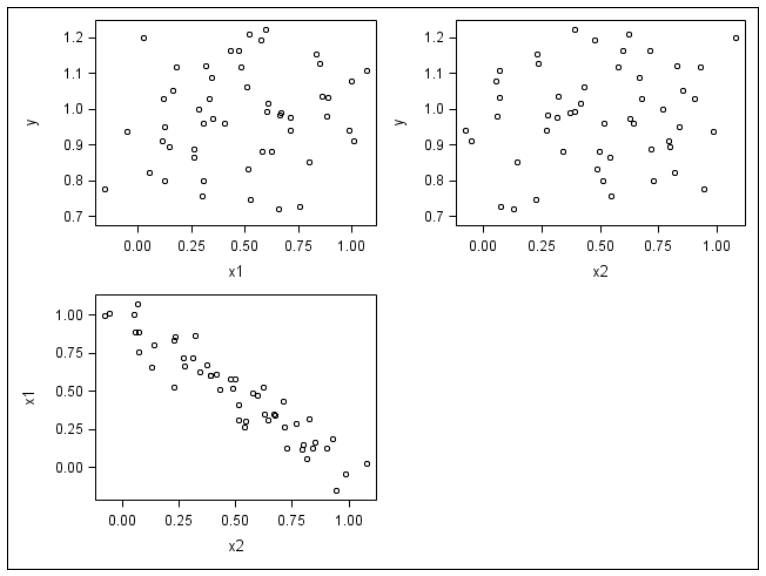
\includegraphics[scale=0.3]{plots/scat}}
\end{frame}

\begin{frame}{\texttt{proc reg} output}
\centerline{$x_1$ important marginally? $Y_i=\beta_0+\beta_1 x_{i1}+\epsilon_i$}

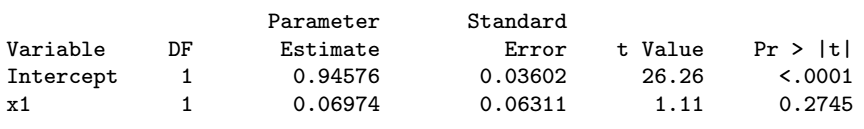
\includegraphics[scale=0.35]{plots/x1}

\centerline{$x_2$ important marginally? $Y_i=\beta_0+\beta_2 x_{i2}+\epsilon_i$}

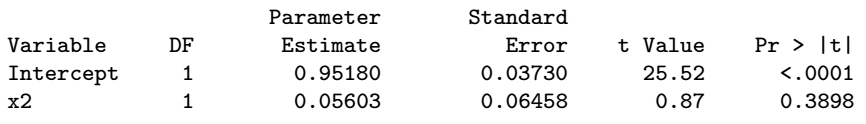
\includegraphics[scale=0.35]{plots/x2}

\centerline{$x_1$, $x_2$ important jointly? $Y_i=\beta_0+\beta_1 x_{i1}+\beta_2 x_{i2}+\epsilon_i$}

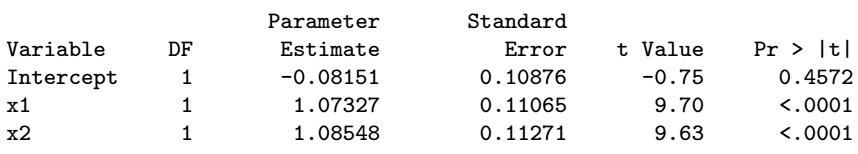
\includegraphics[scale=0.35]{plots/x12}
\end{frame}

\begin{frame}{Nonlinear relationship?}
Marginally, $x_1$ and $x_2$ have highly nonlinear relationships with $Y$. Should we transform?

\centerline{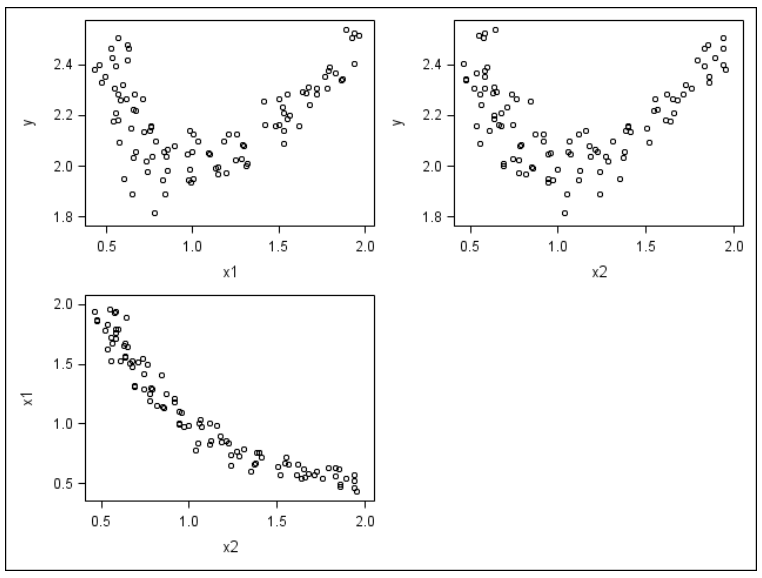
\includegraphics[scale=0.3]{plots/nonlinear}}
\end{frame}

\begin{frame}[fragile]
\frametitle{Regression output}
Let's try fitting a simple main effects model without any transformation.
$$
Y_i=\beta_0 + \beta_1 x_{i1} + \beta_2 x_{i2} + \epsilon_i
$$

\begin{footnotesize}
\begin{verbatim}
                   Parameter     Standard
Variable   DF       Estimate        Error      t Value     Pr > |t|
Intercept   1    -0.00036626      0.00130        -0.28       0.7791
x1          1        1.00022   0.00059936      1668.80       <.0001
x2          1        1.00009   0.00060998      1639.54       <.0001
\end{verbatim}
\end{footnotesize}

both $x_1$ and $x_2$ are important, but does the model fit okay?
\end{frame}


\begin{frame}{Model fit is okay}
\centerline{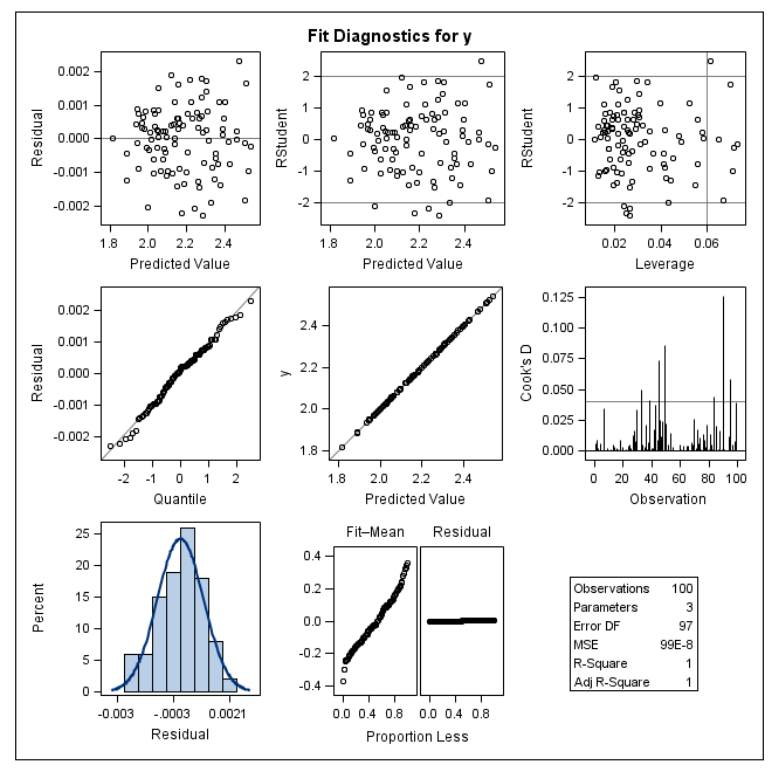
\includegraphics[scale=0.25]{plots/diag}}
\vspace{10pt}

Look at $Y_i$ vs. $\hat{Y}_i$ and $R^2$!
\end{frame}

\begin{frame}{No pattern here, either}
\centerline{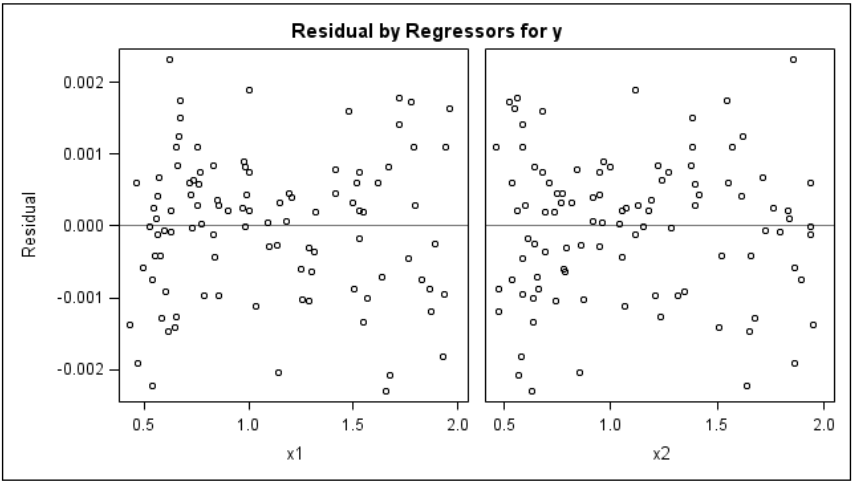
\includegraphics[scale=0.25]{plots/yvsy}}
\end{frame}

\section{Model Building and Types of Studies}

\begin{frame}{9.1 Model building overview (pp.~343--349)}

Book outlines four steps in data analysis:
\begin{enumerate}
\item Data collection and preparation  
\item \pause Reduction of explanatory variables. Mass screening for ``good'' predictors.
\item \pause Model refinement and selection.
\item \pause Model validation.
\end{enumerate}
\vspace{20pt}

\pause The way the data was collected may affect steps 2 \& 3.\\~\\
\pause Model validation should not be confused with model diagnostics (residual analysis).
\end{frame}

\begin{frame}{Data collection strategies}
\begin{itemize}
    \item \textbf{Controlled experiments}: subjects (experimental units) assigned to $x$-levels by experimenter
    \begin{itemize}
        \item<2-> \textbf{Purely controlled experiments}: researcher  uses only predictors that were assigned to units
        \item<3-> \textbf{Controlled experiments with covariates} (uncontrolled variables): researcher has additional predictors associated with units
    \end{itemize}
    \item<4-> \textbf{Observational studies}: subjects have $x$-levels associated with them (not assigned by researcher)
    \begin{itemize}
        \item<5-> \textbf{Confirmatory studies}: it is \textit{hypothesized} that new (primary) predictors are associated with $Y$; \pause while there are predictors, \textit{known} to be associated with $Y$ (called risk factors).
        \item<6-> \textbf{Exploratory studies}: it is hypothesized that some or all of potential predictors are associated with $Y$.
    \end{itemize}
\end{itemize}
\end{frame}


\begin{frame}{Reduction of Explanatory Variables}
\begin{itemize}
    \item Controlled experiments
    \begin{itemize}
        \item\pause Purely controlled experiments: rarely any need or desire to reduce number of predictors
        \item\pause Controlled experiments with covariates: remove any covariates that do not reduce the error variance
    \end{itemize}
    \item\pause Observational Studies
    \begin{itemize}
        \item\pause Confirmatory Studies: Must keep in all risk factors to compare with previous research, should keep all primary variables as well
        \item\pause Exploratory Studies: Often have many potential predictors (and polynomials and interactions). \pause Want to fit parsimonious model that explains much of the variation in $Y$, while keeping model as basic as possible. \pause Caution: one shall not make decisions based on single variable $t$-tests.
    \end{itemize}
\end{itemize}

    
\end{frame}


\begin{frame}{9.2 Surgical unit example}
\begin{itemize}
\item First steps often involve plots:
\begin{itemize}
\item Plots to indicate correct functional form of predictors and/or response.
\item Plots to indicate possible interaction.
\item Exploration of correlation among predictors (maybe).
\item Often a first-order model is a good starting point.
\end{itemize}
\item Once a reasonable set of potential predictors is identified, formal model selection begins.
\item If the number of predictors is large, say $k\ge10$, we can use (automated) stepwise procedures to reduce the number of variables (and models) under consideration.
\end{itemize}
\end{frame}

\begin{frame}{Surgical unit example: predictors}
A hospital surgical unit was interested in predicting survival in patients undergoing a particular type of liver operation. A random selection of 108 patients was available for analysis.
\begin{align*}
X_1\qquad&\text{blood clotting score}\\
X_2\qquad&\text{prognostic index}\\
X_3\qquad&\text{enzyme function test score}\\
X_4\qquad&\text{liver function test score}\\
\ldots
\end{align*}
\centerline{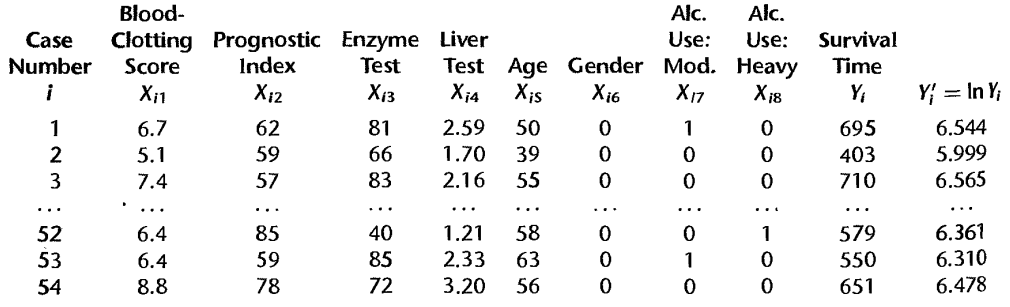
\includegraphics[scale=0.25]{plots/dataset}}
\end{frame}

\begin{frame}{Surgical unit example: residual plots}
\centerline{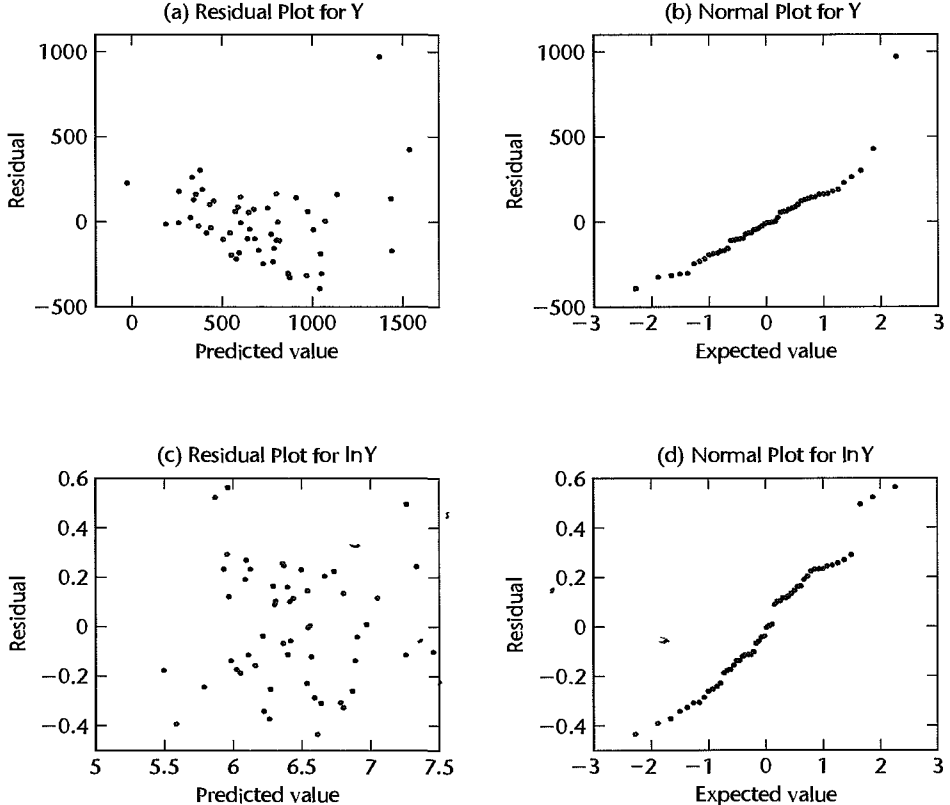
\includegraphics[scale=0.27]{plots/res-y}}
\end{frame}

\begin{frame}{Surgical unit example: scatterplot matrix}
\centerline{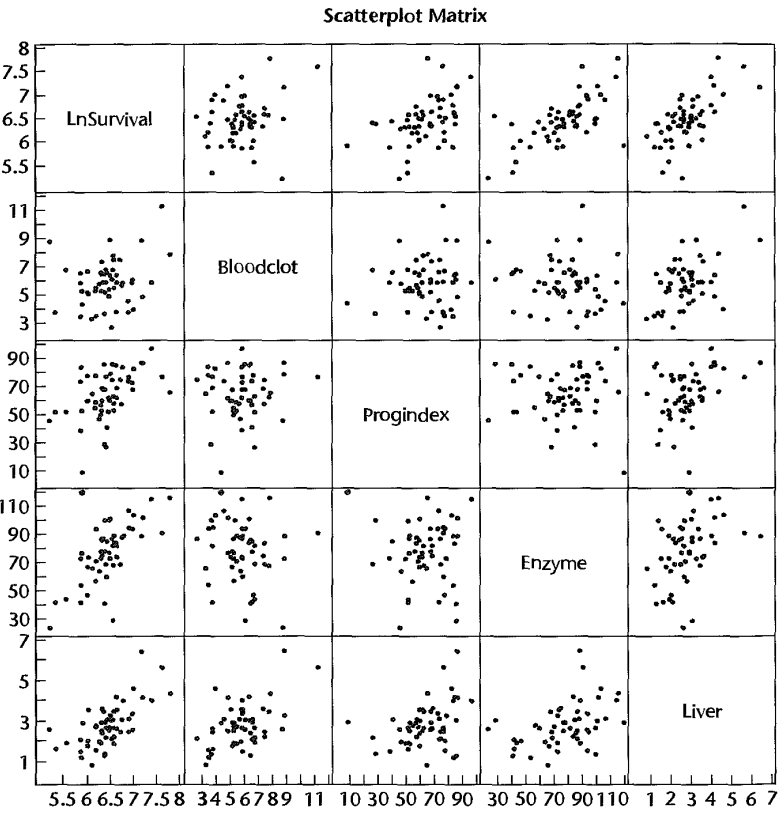
\includegraphics[scale=0.27]{plots/scat-mat}}
\end{frame}

\section{Model Selection}

\begin{frame}{9.3: Model selection}
Once we reduce the set of potential predictors to a reasonable
number, we can examine all possible models and choose the ``best''
according to some criterion.
\vspace{10pt}

\pause Say we have $k$ predictors $x_1$, \ldots, $x_k$ and we want to find a good subset of predictors that predict the data well. There are several
useful criteria to help choose a subset of predictors.
\end{frame}

\begin{frame}{Adjusted-$R^2$, $R_a^2$}
\begin{small}
%``Regular'' $R^2$ measures how well the model predicts the data that built it. It is possible to have a model with $R^2=1$ (predicts the data that built it perfectly), but has \textit{lousy out-of-sample prediction}.
%\vspace{10pt}

The \textit{adjusted} $R^2$, denoted $R_a^2$ ``fixes'' $R^2$ to provide a measure of how good the  model will predict data not used to build the model. For a candidate model with $p-1$ predictors
$$
R^2_a=1-\frac{\text{SSE}/(n-p)}{\text{SSTO}/(n-1)}\pause\quad\left(=1-\frac{\text{MSE}}{S^2_Y}\right).
$$
\begin{itemize}
\item<2-> Equivalent to choosing the model with the \textit{smallest} $\text{MSE}$.
\item<3-> If irrelevant variables are added, $R_a^2$ may decrease unlike ``regular'' $R^2$ ($R^2_a$ can be negative!).
\item<4-> $R_a^2$ penalizes model for being too complex.
\item<5-> Problem: $R_a^2$ is greater for a ``bigger'' model whenever the
F-statistic for comparing bigger to smaller is greater than 1 (\textbf{show this}). \onslide<6->{We usually want F-statistic to be a \textit{lot} bigger than 1 before
adding in new predictors}\onslide<7->{\quad $\Rightarrow$\quad \textit{too liberal}.}
\end{itemize}
\end{small}
\end{frame}

\begin{frame}{Akaike Information Criterion}
In general, \textbf{Akaike Information Criterion (AIC)} is
$$
\text{AIC}=-2\ln L(\hat{\boldsymbol\theta})+2p
$$
for a model with parameters $\boldsymbol\theta\in\mathbb{R}^p$ and likelihood function $L$.

\pause\begin{exe}
Show that for the MLR with normal errors,
$$
\text{AIC} = n\ln(\text{SSE})+2p + C
$$
where $C$ is a constant that does not depend on SSE and $p$.
\end{exe} 
\begin{itemize}
\item\pause $2p$ is ``penalty'' term for adding predictors.
\item\pause Like $R_a^2$, AIC favors models with small SSE, but penalizes models with too many variables $p$.
\item\pause $\Rightarrow$ Between two models, we prefer the one with lower AIC.
\end{itemize}
\end{frame}

\begin{frame}{Bayesian
Information Criterion}
In general, \textbf{Bayesian
Information Criterion (BIC)} is
$$
\text{BIC}=-2\ln L(\hat{\boldsymbol\theta})+p\ln(n)
$$
\pause\begin{exe}
Show that for the MLR with normal errors,
$$
\text{BIC} = n\ln(\text{SSE}) + p\log(n) + C
$$
\end{exe}
\pause\begin{itemize}
\item BIC is similar to AIC, but for $n\ge8$, the BIC ``penalty term'' is
more severe.
\end{itemize}
\end{frame}


\begin{frame}{Mallow's $C_p$}
Full model with $k$ predictors and Reduced model with $p - 1$ predictors. \pause \textbf{Mallow's $C_p$} is
$$
C_p=\frac{\text{SSE}(\text{Reduced})}{\text{MSE}(\text{Full})}-n+2p
$$
\begin{itemize}
\item\pause Estimates $\frac{\E[\hat{Y}_i-\E[Y_i]]^2}{\sigma^2}$, where $\hat{Y}_i$ is from the Reduced model (pp. 357--359).
\item\pause Recall that $\E[\text{MSE}(\text{Full})]=\sigma^2$
\item\pause If the Reduced model is unbiased, i.e. $\E[\text{MSE}(\text{Reduced})]=\sigma^2$, \pause then $\E[\text{SSE}(\text{Reduced})]=(n-p)\sigma^2$, \pause and
$$
C_p\approx\frac{(n-p)\sigma^2}{\sigma^2}-n+2p=p
$$
\item\pause The Full model always has $C_{k+1} = k + 1$.
\end{itemize}
\end{frame}

\begin{frame}{Mallow's $C_p$}
If $C_p \approx p$ then the reduced model predicts as well as the full model. If $C_p < p$ then the reduced model is estimated to
be less \textit{biased} than the full model.

\begin{figure}
    \centering
    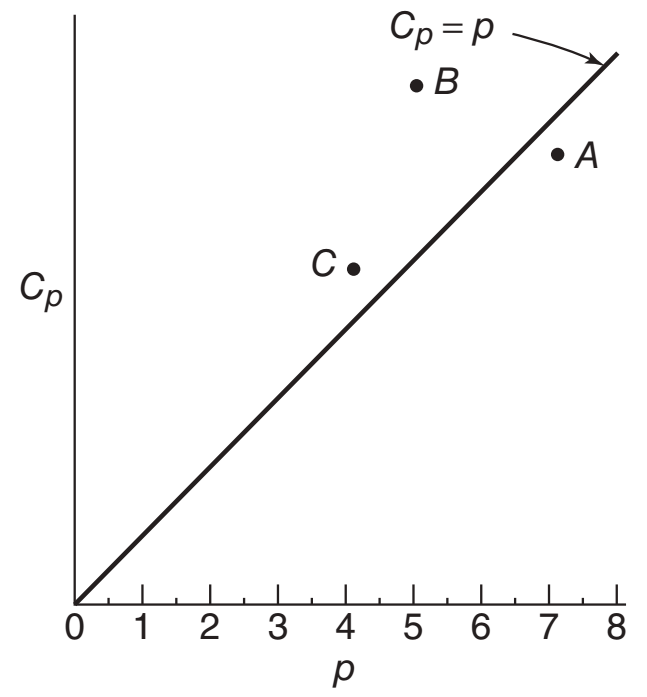
\includegraphics[height=.4\textheight]{plots/mallows_cp.png}
    \caption{A $C_p$ plot}
\end{figure}

\pause In practice, just choose model with smallest $C_p$.
\end{frame}

\begin{frame}{Which criteria to use?}
$R_a^2$, AIC, BIC, and $C_p$ may give different ``best'' models, or they
may agree. Ultimate goal is to find model that balances:
\begin{itemize}
\item\pause A good fit to the data.
\item\pause Low bias.
\item\pause Parsimony.
\end{itemize}
All else being equal, the simpler model is often easier to interpret
and work with. Christensen (1996) recommends $C_p$ and notes the
similarity between $C_p$ and AIC.
\end{frame}

\begin{frame}{Methods for ``automatically'' picking variables}
\begin{itemize}
\item Any regression textbook will caution against not thinking
about the data at all and simply using automated procedures.
\item\pause Automated procedures \textit{cannot} assess a good functional form for a predictor, \textit{cannot} think about which interactions might be important, etc.
\item\pause Anyway, automated procedures are widely used and \textit{can} produce good models. \pause But they can also produce models that are \textit{substantially inferior} to other models built from the same predictors using scientific input and common sense.
\end{itemize}
\end{frame}

\begin{frame}[fragile]{Example: cruise ships}{\url{https://github.com/zh3nis/MATH440/blob/main/chp09/cruise.R}}
A cruise ship company wishes to model the \texttt{crew size} needed for a ship using predictors such as: \texttt{age}, \texttt{tonnage}, \texttt{passengers}, \texttt{length}, \texttt{cabins} and passenger density (\texttt{passdens}). 

\pause
\begin{tiny}
\begin{verbatim}
> cruise <- read.fwf("http://www.stat.ufl.edu/~winner/data/cruise_ship.dat", ...)
> head(cruise)
         ship      cline age tonnage passengers length cabins passdens  crew
1 Journey        Azamara   6  30.277       6.94   5.94   3.55    42.64  3.55
2 Quest          Azamara   6  30.277       6.94   5.94   3.55    42.64  3.55
3 Celebration   Carnival  26  47.262      14.86   7.22   7.43    31.80  6.70
4 Conquest      Carnival  11 110.000      29.74   9.53  14.88    36.99 19.10
5 Destiny       Carnival  17 101.353      26.42   8.92  13.21    38.36 10.00
6 Ecstasy       Carnival  22  70.367      20.52   8.55  10.20    34.29  9.20
\end{verbatim}
\end{tiny}

\pause Without concerning ourselves with potential interactions we will look at simple additive models.
\end{frame}

\begin{frame}[fragile]{Cruise ships --- Full model}
\begin{tiny}
\begin{verbatim}
> fit0 = lm(crew ~ age + tonnage + passengers + length + cabins + passdens, data=cruise)
> summary(fit0)

Call:
lm(formula = crew ~ age + tonnage + passengers + length + cabins + 
    passdens, data = cruise)

Residuals:
    Min      1Q  Median      3Q     Max 
-1.7700 -0.4881 -0.0938  0.4454  7.0077 

Coefficients:
              Estimate Std. Error t value Pr(>|t|)    
(Intercept) -0.5213400  1.0570350  -0.493  0.62258    
age         -0.0125449  0.0141975  -0.884  0.37832    
tonnage      0.0132410  0.0118928   1.113  0.26732    
passengers  -0.1497640  0.0475886  -3.147  0.00199 ** 
length       0.4034785  0.1144548   3.525  0.00056 ***
cabins       0.8016337  0.0892227   8.985 9.84e-16 ***
passdens    -0.0006577  0.0158098  -0.042  0.96687    
---
Signif. codes:  0 ‘***’ 0.001 ‘**’ 0.01 ‘*’ 0.05 ‘.’ 0.1 ‘ ’ 1

Residual standard error: 0.9819 on 151 degrees of freedom
Multiple R-squared:  0.9245,	Adjusted R-squared:  0.9215 
F-statistic:   308 on 6 and 151 DF,  p-value: < 2.2e-16        
\end{verbatim}
\end{tiny}
\end{frame}


\begin{frame}[fragile]
\frametitle{Best subsets}
\begin{tiny}
\begin{verbatim}
> library(leaps)
> allcruise <- regsubsets(crew ~ age + tonnage + passengers + length + cabins + passdens, 
+                         nbest=4, data=cruise)
> all_output <- summary(allcruise)
> with(all_output, round(cbind(which, rsq, adjr2, cp, bic), 3))
  (Intercept) age tonnage passengers length cabins passdens   rsq adjr2      cp      bic
1           1   0       0          0      0      1        0 0.904 0.903  37.772 -360.238
1           1   0       1          0      0      0        0 0.860 0.859 125.086 -300.954
1           1   0       0          1      0      0        0 0.838 0.837 170.523 -277.122
1           1   0       0          0      1      0        0 0.803 0.801 240.675 -246.201
2           1   0       0          0      1      1        0 0.916 0.915  15.952 -376.131
2           1   0       0          0      0      1        1 0.912 0.911  24.261 -368.502
2           1   0       1          0      0      1        0 0.911 0.909  26.792 -366.249
2           1   0       0          1      0      1        0 0.908 0.907  32.443 -361.332
3           1   0       0          1      1      1        0 0.922 0.921   5.857 -382.878
3           1   0       0          0      1      1        1 0.919 0.918  11.341 -377.413
3           1   0       1          1      0      1        0 0.918 0.916  14.023 -374.808
3           1   1       0          0      1      1        0 0.917 0.915  15.909 -373.002
4           1   0       1          1      1      1        0 0.924 0.922   3.847 -381.933
4           1   1       0          1      1      1        0 0.923 0.921   5.084 -380.652
4           1   0       0          1      1      1        1 0.923 0.921   5.197 -380.534
4           1   0       1          0      1      1        1 0.919 0.917  13.056 -372.631
5           1   1       1          1      1      1        0 0.924 0.922   5.002 -377.752
5           1   0       1          1      1      1        1 0.924 0.922   5.781 -376.939
5           1   1       0          1      1      1        1 0.924 0.921   6.240 -376.462
5           1   1       1          0      1      1        1 0.920 0.917  14.904 -367.717
6           1   1       1          1      1      1        1 0.924 0.921   7.000 -372.692
\end{verbatim}
\end{tiny}
\pause A good model choice might be the model with 4 predictors: tonnage, passengers, length, and cabins, whose $R_a^2 = 0.922$, $C_p = 3.847$, and
$\text{BIC}= −381.933$. %Also we note that this model's AIC is lower than that of the full model.
\end{frame}

\begin{frame}[fragile]{AIC full vs reduced}
\begin{verbatim}
> fit3 <- update(fit0, . ~ . - age - passdens)
> AIC(fit3)
[1] 448.3229
> AIC(fit0)
[1] 451.4394    
\end{verbatim}
\end{frame}

\begin{frame}{9.4 Automated variable search}
As discussed, it is possible to have a large set of predictor variables (including
interactions). The goal is to fit a ``parsimoneous'' model that explains as
much variation in the response as possible with a relatively small set of
predictors.\\~\\

\pause There are 3 automated procedures
\begin{itemize}
    \item\pause Backward Elimination (Top down approach)
    \item\pause Forward Selection (Bottom up approach)
    \item\pause Stepwise Regression (Combines Forward/Backward)
\end{itemize}

\pause We will explore these procedures using two different elimination/selection
criteria. \pause One that uses t-test and p-value and another that uses the AIC
value.
\end{frame}

\begin{frame}{Backward elimination}
\begin{enumerate}
\item Select a significance level to \textit{stay} in the model (e.g. $\alpha_s = 0.20$, generally
.05 is too low, causing too many variables to be removed).
\item\pause Fit the full model with all possible predictors.
\item\pause Consider the predictor with lowest t-statistic (highest p-value).
\begin{itemize}
    \item\pause If p-value $> \alpha_s$, remove the predictor and fit model without this
variable (must re-fit model here because partial regression coefficients change). 
    \item\pause If p-value $\le \alpha_s$, stop and keep current model.
\end{itemize}
\item\pause Continue until all predictors have p-values $\le\alpha_s$.    
\end{enumerate}
\end{frame}

\begin{frame}{Forward selection}
\begin{enumerate}
    \item Select a significance level to \textit{enter} the model (e.g. $\alpha_e = 0.20$, generally .05 is too low, causing too few variables to be entered).
\item\pause Fit all simple regression models.
\item\pause Consider the predictor with the highest t-statistic (lowest p-value).
\begin{itemize}
    \item\pause If p-value $\le\alpha_e$, keep this variable and fit all two variable models
that include this predictor.
    \item\pause If p-value $>\alpha_e$, stop and keep previous model.
\end{itemize}
\item\pause Continue until no new predictors have p-values $\le\alpha_e$.    
\end{enumerate}
\end{frame}

\begin{frame}{Stepwise regression}
\begin{enumerate}
\item Select $\alpha_s$ and $\alpha_e$, ($\alpha_e < \alpha_s$).
\item\pause  Start like Forward Selection (bottom up process) where new variables
must have p-value $\le\alpha_e$ to enter.
\item\pause Re-test all ``old variables'' that have already been entered, must have
p-value $\le\alpha_s$ to stay in model.
\item\pause Continue until no new variables can be entered and no old variables
need to be removed.
\end{enumerate}
\end{frame}


\begin{frame}[fragile]{Backward and Forward for cruise ships}
\begin{scriptsize}
\begin{verbatim}
> library(olsrr)
> ols_step_backward_p(fit0)

                          Elimination Summary                            
------------------------------------------------------------------------
        Variable                  Adj.                                      
Step    Removed     R-Square    R-Square     C(p)       AIC        RMSE     
------------------------------------------------------------------------
   1    passdens      0.9245       0.922    5.0017    449.4412    0.9786    
   2    age            0.924      0.9221    3.8468    448.3229    0.9782    
------------------------------------------------------------------------

> ols_step_forward_p(fit0)

                             Selection Summary                              
---------------------------------------------------------------------------
        Variable                    Adj.                                       
Step     Entered      R-Square    R-Square     C(p)        AIC        RMSE     
---------------------------------------------------------------------------
   1    cabins          0.9041      0.9034    37.7724    479.2060    1.0886    
   2    length          0.9160      0.9149    15.9524    460.2507    1.0221    
   3    passengers      0.9220      0.9205     5.8566    450.4411    0.9878    
   4    tonnage         0.9240      0.9221     3.8468    448.3229    0.9782    
---------------------------------------------------------------------------
\end{verbatim}
\end{scriptsize}    
\end{frame}

\begin{frame}[fragile]{Stepwise procedure for cruise ships}
\begin{tiny}
\begin{verbatim}
> ols_step_both_p(fit0)

                              Stepwise Selection Summary                                
---------------------------------------------------------------------------------------
                       Added/                   Adj.                                       
Step     Variable     Removed     R-Square    R-Square     C(p)        AIC        RMSE     
---------------------------------------------------------------------------------------
   1      cabins      addition       0.904       0.903    37.7720    479.2060    1.0886    
   2      length      addition       0.916       0.915    15.9520    460.2507    1.0221    
   3    passengers    addition       0.922       0.921     5.8570    450.4411    0.9878    
   4     tonnage      addition       0.924       0.922     3.8470    448.3229    0.9782    
---------------------------------------------------------------------------------------    
\end{verbatim}
\end{tiny}
\end{frame}

\section{Model Validation (briefly)}

\begin{frame}{PRESS$_p$ criterion}
$$
\text{PRESS}_p = \sum_{i=1}^n(Y_i-\hat{Y}_{i(i)})^2\quad \left(=\sum_{i=1}^n\left[\frac{e_i}{1-h_{ii}}\right]^2\right),
$$
where $\hat{Y}_{i(i)}$ is the fitted value at $\mathbf{x}_i$ with the $(\mathbf{x}_i, Y_i)$ omitted.
\begin{itemize}
\item\pause This is leave-one-out prediction error. The smaller, the better.
\item\pause Having $\text{PRESS}_p \approx \text{SSE}_p$ supports the \textit{validity} of the model
with $p$ predictors (p.~374). 
\end{itemize}
\end{frame}

\begin{frame}{Caveats for automated procedures}
\begin{itemize}
\item There is no ``best'' way to search for good models.
\item\pause There may be \textit{several} ``good'' models.
\item\pause If you use the same data to \textit{estimate} the model and \textit{choose}
the model, the regression effects are \textit{biased}!
\textit This leads to the idea of data splitting; one portion of the data
is the \textit{training data} and the other portion is the \textit{validation set}
(Section 9.6, p.~372). $\text{PRESS}_p$ can also be used.
\end{itemize}
\end{frame}

\end{document}